\section{System Design and Algorithms} \label{sec:Algorithms}

\begin{figure}
\centering
    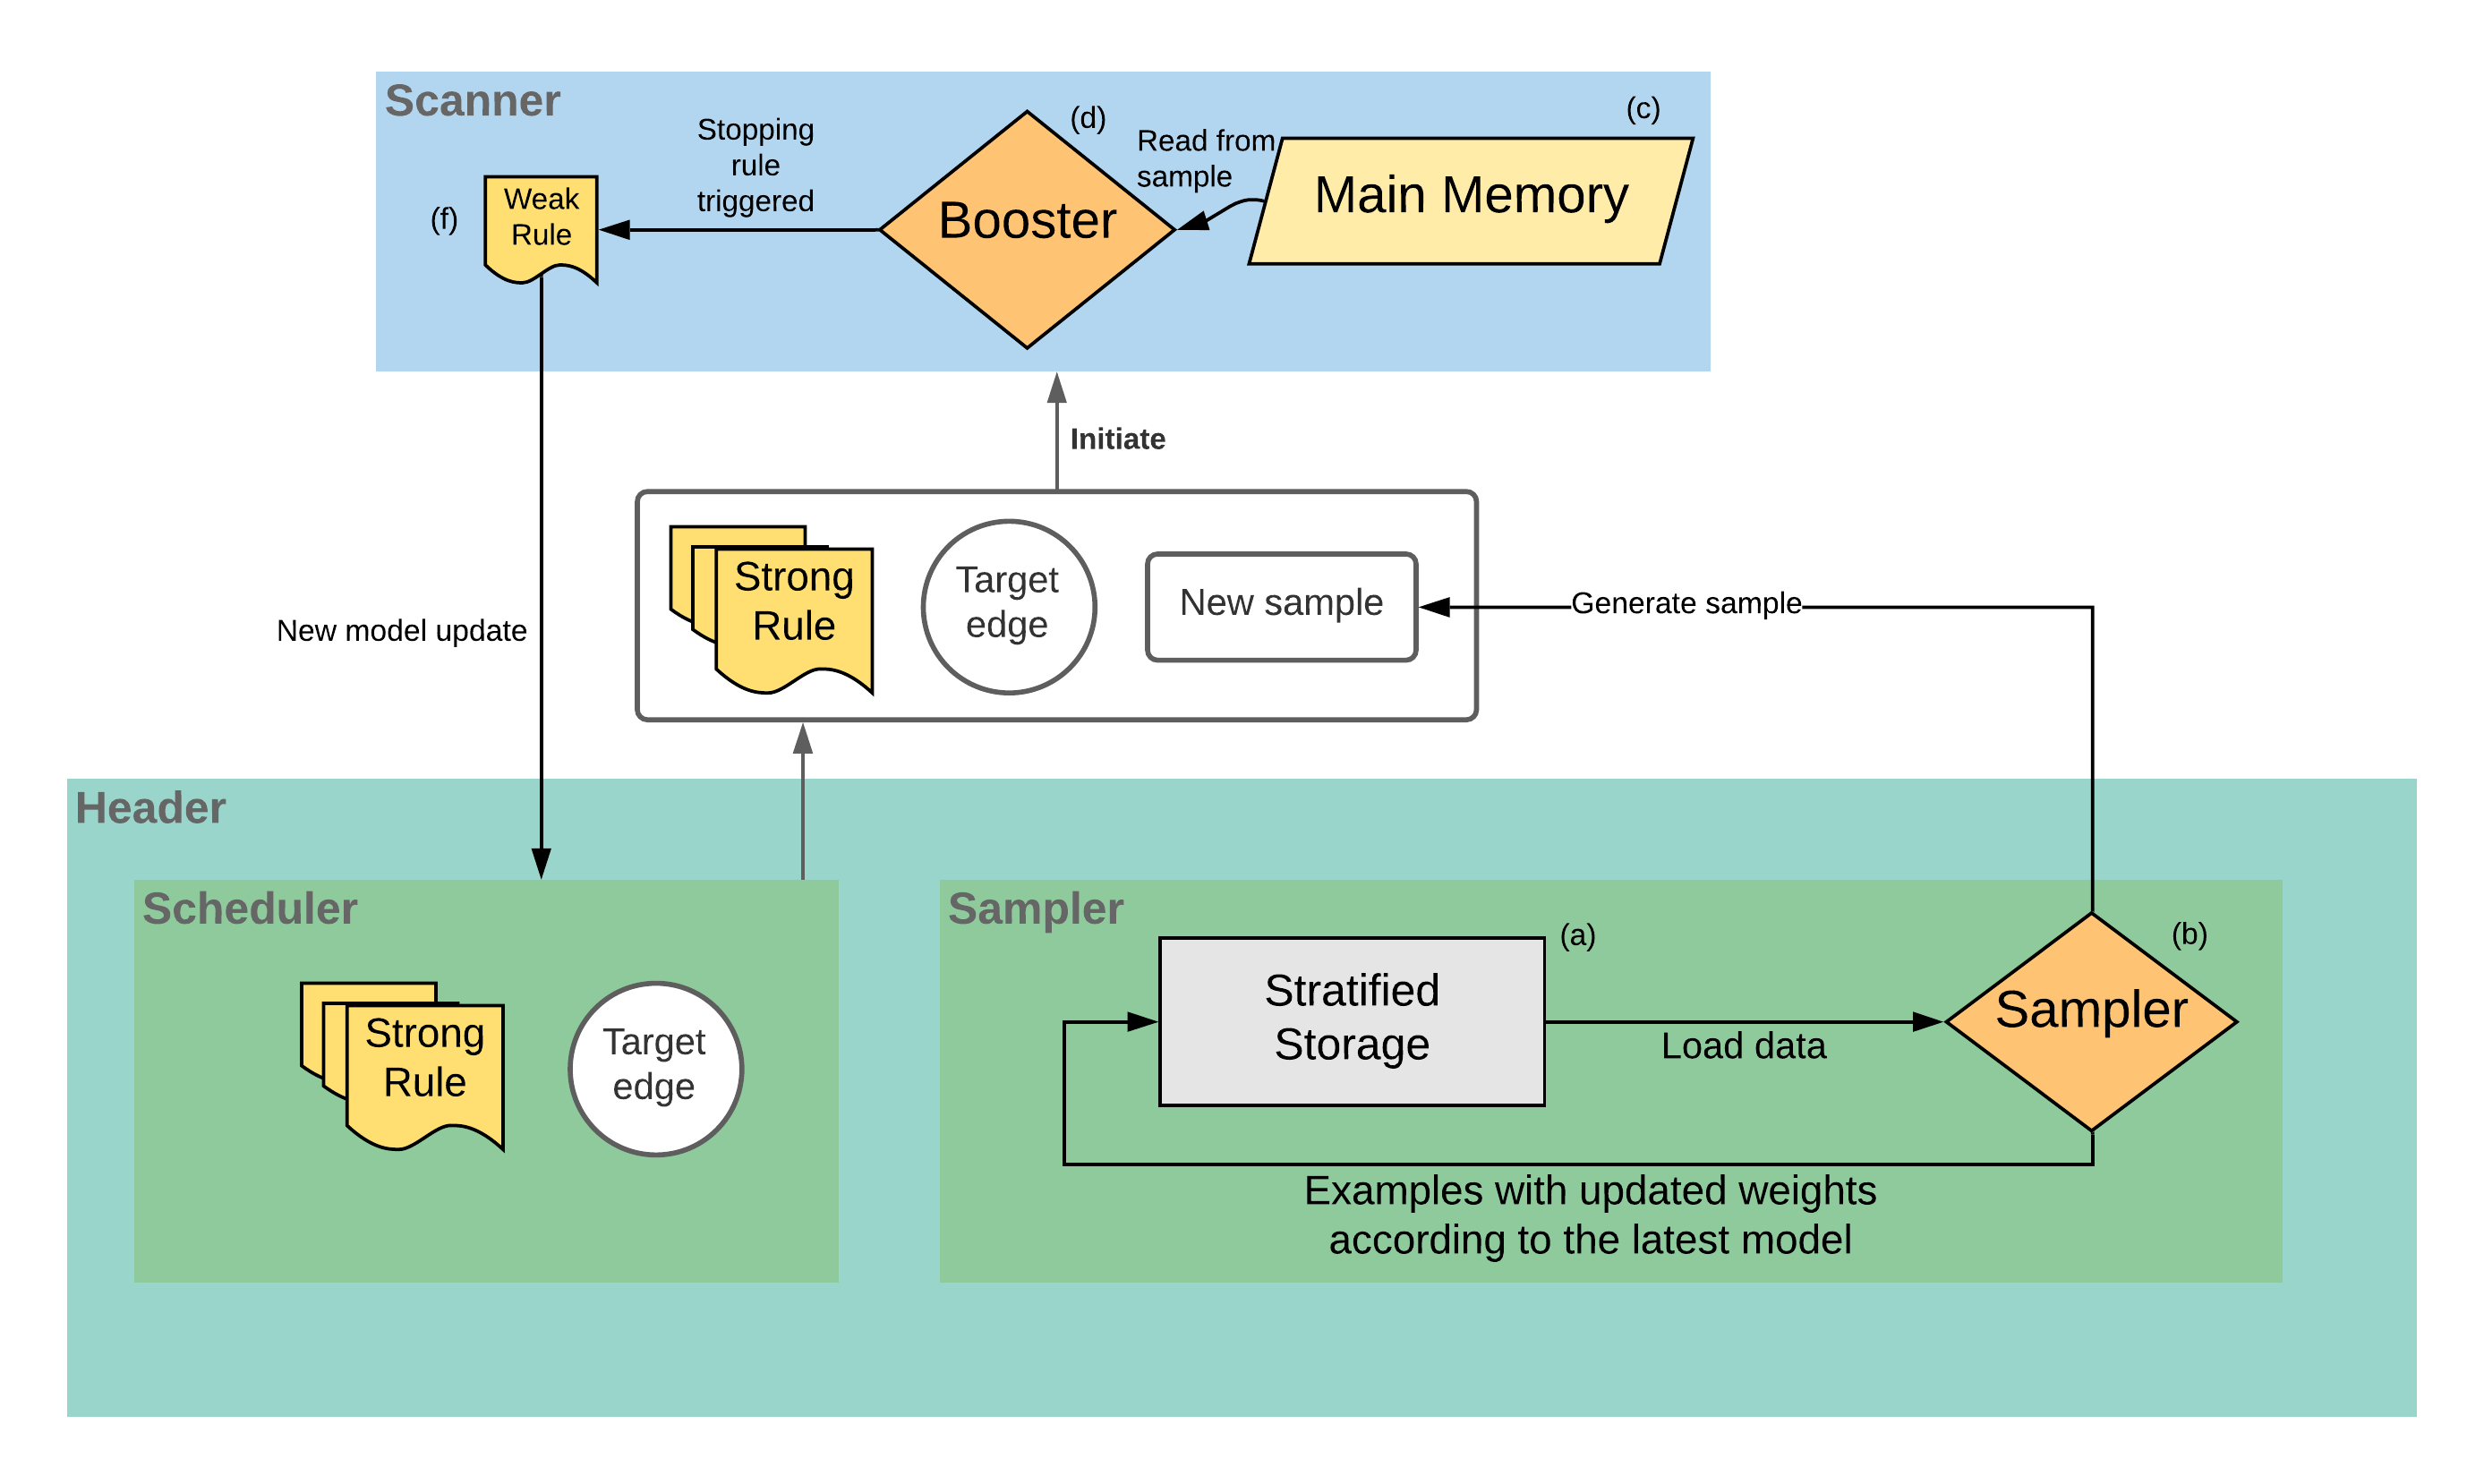
\includegraphics[width=0.5\textwidth]{figs/HeaderScanner.png}
    \caption{The \Sparrow\ system architecture.}\label{fig:architecture}
    \vspace{0pt}
%\end{minipage}
\end{figure}

In this section we describe \Sparrow.

The main procedure of \Sparrow\ is for identifying a rule that has a significant
edge (Equation~\ref{eqn:true-edge}). There are two
subroutines that can execute in parallel in the process: a
{\bf Header } and multiple {\bf Scanners}. We describe each subroutine in turn.


\subsection*{Scanner}

The task of a scanner (element {\bf (d)} in Figure~\ref{fig:architecture})
is to read training examples sequentially and stop
when it has identified one of the rules to be a {\em good} rule.
It is is initiated by the Header given 3 parameters: (1) current
strong rule $H_t$, (2) target edge $\gamma_t$ which is the threshold
that defines a {\em good} rule, and (3) a sample from the training data.

More specifically, at any time point the scanner stores the current strong
rule $H_t$, a set of candidate weak rules $\weakRules$ (which
define the candidate strong rules), and a target
edge $\gamma_t$. The scanner scans the training examples stored in
memory sequentially, one at a time. It computes the weight of the
examples using $H_t$ and then updates a running estimate of the edge
of each weak rule $h \in \weakRules$.

The scan stops when the stopping rule determine that
the true edge of a particular weak rule
$\gamma(h_t)$ is, with high probability,
larger than a threshold $\gamma$. The
worker then adds the identified weak rule $h_t$ {\bf (f)} to the current
strong rule $H_t$ to create a new strong rule $H_{t+1}$.
The weight of the added rule is calculated assuming that its edge is
equal to $\gamma$.

The scanner falls into the \textit{Failed} status if after exhausting
all examples in the current sample set, no weak rule with an advantage
larger than the threshold $\gamma$ is detected.

When a scanner terminates, it communicates either the newly accepted
weak rule or a \textit{Failed} message back to the Header.
The Header then updates the strong rule and the target edge accordingly.


\subsection*{Header}

The Header plays a rule similar to the Parameter Server. It consists
of two components, a Scheduler and a Sampler.


The Scheduler maintains a global model. It receives the model updates from scanners, and decides whether or not accepting the updates to the global model. If it accepts the model update, the Scheduler updates the global model accordingly, and broadcast the new global model to all Scanners. If the model updates is incompatible with the global model, for example, if it is based on an out-dated global model version, the Scheduler would reject the model updates.

The Scheduler also maintains the value of
the targeted edge $\gamma$. If no scanner finds a new model update for a long period of time, the Scheduler decreases the value of the targeted edge, and broadcast the new value.

Our assumption is that the entire training dataset does
not fit into main memory and is therefore stored in external storage
{\bf (a)}. As boosting progresses, the weights of the examples become
increasingly skewed, making the dataset in memory effectively smaller.
To counteract that skew, {\bf Sampler} prepares a {\em new}
training set, in which all of the examples have equal weight, by using
selective sampling. When the effective sample size associated
with the old training set becomes too small, the scanner stops using
the old training set and starts using the new one.\footnote{The
  sampler and scanner can run in parallel on separate cores. However in
  our current implementation the worker alternates between scanning and
  sampling.}


The Sampler uses selective sampling by which we mean that the
probability that an example $(x,y)$ is added to the sample is
proportional to $w(x,y)$. Each added example is assigned an initial
{\bf weight} of $1$.
{There are several known algorithms
  for selective sampling. The best known one is rejection sampling
  where a biased coin is flipped for each example. We use a method
  known as \textit{minimal variance sampling}~\cite{kitagawa_monte_1996}
  because it produces less variation in the sampled set.}
  
\paragraph*{Incremental Updates} Our experience shows that the most
time consuming part of our algorithms is the computation of the
predictions of the strong rules $H_t$. A natural way to reduce this
computation is to perform it incrementally. In our case this is
slightly more complex than in XGBoost or LightGBM, because {\bf
  Scanner} scans only a  fraction of the examples at each
iteration. To implement incremental update we store for each example,
whether it is on disk or in memory, the results of the latest
update. Specifically, we store for each training example the tuple
$(x, y, w_s, w_l,H_l)$, Where $x,y$ are the feature vector and the
label, $H_l$ is the strong rule last used to calculate the weight of
the example. $w_l$ is the weight last calculated, and $w_s$ is
example's weight when it was last sampled by the sampler. In this way
{\bf Scanner} and {\bf Sampler} share the burden of computing
the weights, a cost that turns out to be the lion's share of the total
run time for our system.




\section{Tuning a good policy to set $\gamma$}

The main challenge of Sparrow is to adjust the value of $\gamma$ at a right pace.

We compare Sparrow on the splice site
dataset same as ~\cite{alafate_sparrow_2019},
and use LightGBM as the baseline.
In Figure~\ref{fig:rapid-gamma},
we show a 5x speed-up from using 1 scanner to
using 10 scanners, but the speed-up is not significant when we increase from 10 scanners to 50 scanners.

Current policy for adjusting gamma is not robust. The header node decreases
the value of gamma when a certain number of scanners failed to trigger stopping
rules.
If the values of gamma decrease too fast, we risk converging to a sub-optimal loss.
In Figure~\ref{fig:rapid-gamma}, the green curve corresponds to the setting
where the values of $\gamma$ decrease too fast.
The green curve (trained with 50 scanners) decreases faster than the orange curve (trained with 10 scanners).
The value of gamma decreases every time it sees a fixed number of failures, where a failure is defined as a packet from any scanner saying that the stopping rule failed to trigger after scanning all samples. With more scanners, the head node received more failure packets, and decreased the value of gamma more aggressively.

On the other hand, if the values of $\gamma$ decreases too conservatively,
it could take a very long time to find the right value of $\gamma$ which can trigger the stopping rule.

\begin{figure}
\centering
    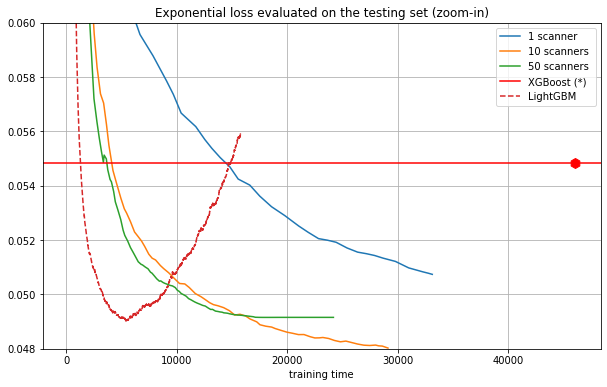
\includegraphics[width=0.5\textwidth]{paper/figs/stale.png}
    \caption{The decrease of loss stales when we decreases the value of gamma too rapidly.}\label{fig:rapid-gamma}
    \vspace{0pt}
%\end{minipage}
\end{figure}

One other problem with asynchronous distributed training is that
with more scanners, we are more likely to find a wrong weak by chance.
In Figure~\ref{fig:overfit},
the green curve starts to perform worse on the test set as the result of overfitting
to the sample set from the training data.
With more scanners we are more likely to find a bad tree. If we then assign a large $\gamma$ to the
bad tree, the performance on the test suffers.

\begin{figure}
\centering
    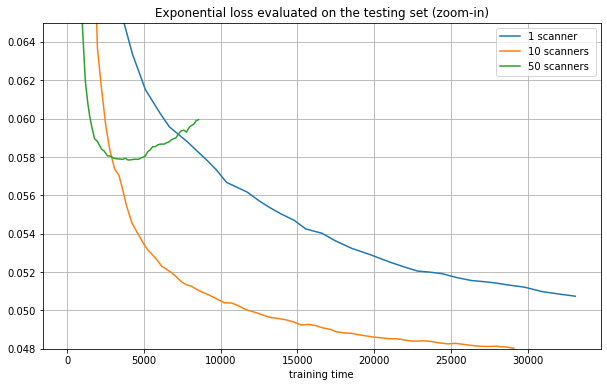
\includegraphics[width=0.5\textwidth]{paper/figs/overfit.png}
    \caption{The weak rule could over-fit to the sampled data when we decreases the value of gamma too slowly.}\label{fig:overfit}
    \vspace{0pt}
%\end{minipage}
\end{figure}